\documentclass{beamer}
%\documentclass[notes]{beamer}
%\documentclass[notes=only]{beamer}
%\documentclass[handout]{beamer}
\usepackage[utf8]{inputenc}
\usetheme{Ilmenau}
\usepackage[frenchb]{babel}    % le documents est en français
\usepackage{amsmath}           % un packages mathématiques
\usepackage{xcolor}            % pour définir plus de couleurs 
\usepackage{graphicx}          % pour insérer des figures
%\usepackage{handoutWithNotes}
%\pgfpagesuselayout{1 on 1 with notes landscape}[a4paper,border shrink=5mm]

		
\usepackage{Slides_08092010}

  \title{Amélioration de la réactivité des réseaux pair à pair pour les MMOGs}
  \author{Xavier Joudiou,\\\tiny{Encadré par: S.Legtchenko \& S.Monnet}}\institute{Université Paris VI, Master SAR}
 % \logo{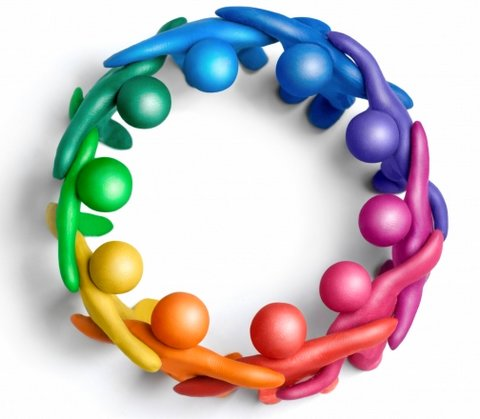
\includegraphics[scale=0.5]{./Ressources/Images/P2P.png}}
  \date{8 Septembre 2010}

  \begin{document}

  \begin{frame}
  \maketitle
  \end{frame}


  \begin{frame}
  \tableofcontents
  \end{frame}

  \section{Introduction}
  \begin{frame}
  	Présentation des points importants à la compréhension des solutions:\\
	\begin{itemize}
		\item Architecture pair à pair Vs Client-Serveur\\
		\item Définition d'un Overlay\\
	\end{itemize}
  \end{frame}

  \begin{frame}
	Architecture pair à pair Vs Client/Serveur\\
	\begin{figure}
	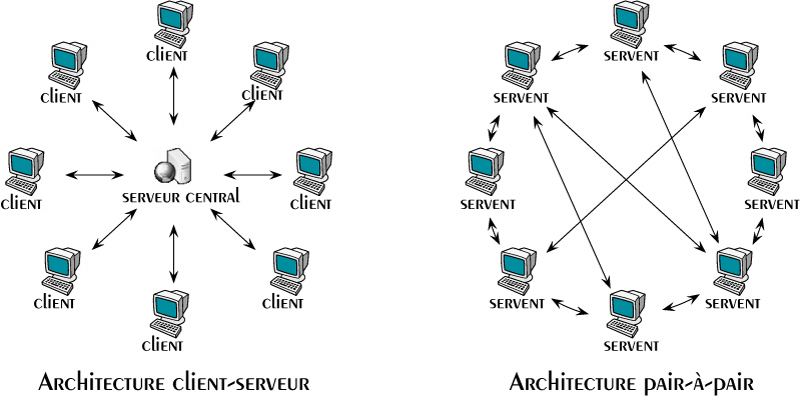
\includegraphics[scale=0.3]{./Ressources/Images/p2p-85145.png}\\
        \label{P2PvsClServ}
        \end{figure}
  \end{frame}
  
  \begin{frame}
	
	\center{Définition d'un Overlay}
 	\begin{columns}
          \begin{column}{5cm}
          	Un Overlay est un réseau informatique formant un graphe où les liens sont déterminés avec un critère logique.\\
	  \end{column}
          \begin{column}{5cm}
        	\begin{figure}
        	  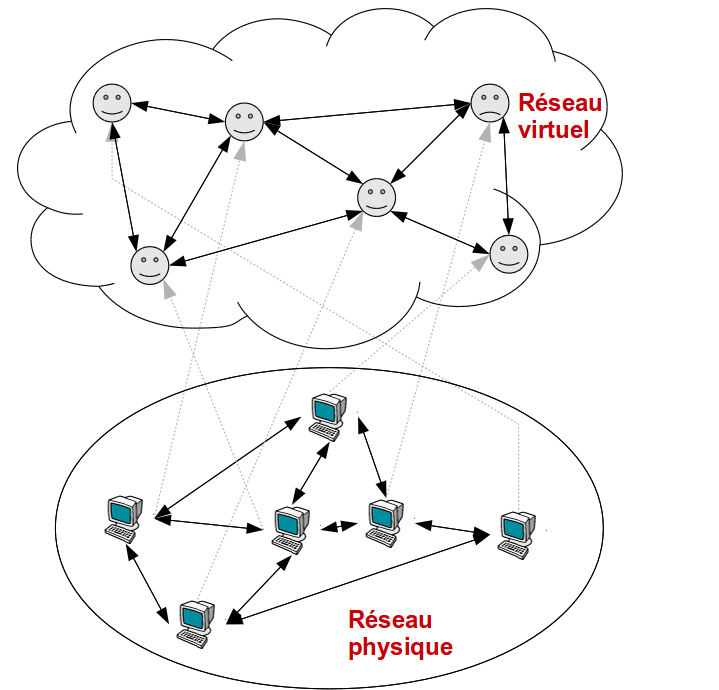
\includegraphics[scale=0.2]{./Ressources/Images/overlay.png}\\
        	  \label{Propa_Algo}
        	\end{figure}
          \end{column}
        \end{columns}
	
  \end{frame}
	
  \section{État de l'art}
  \begin{frame}
	Présentation des différents mécanismes importants pour la compréhension des solutions introduites:\\
	\begin{itemize}
		\item Solipsis\\
		\item Étude des traces des joueurs de MMOG\\
		\item Blue Banana \\
	\end{itemize}
  \end{frame}

  \subsection{Solipsis}

  \begin{frame}
	Solipsis:\\
	\begin{itemize}
		\item propose un monde virtuel entièrement décentralisé et scalable\\
		\item met en place un overlay avec une forte malléabilité applicative\\
		\item chaque entité collecte des informations pour reconstituer son environnement local.\\
	\end{itemize}
  \end{frame}

  \begin{frame}
	Solipsis introduit plusieurs propriétés:
	\begin{itemize}
                \item \textit{Local Awareness:}\\
                Une entité doit être connectée avec tous ses plus proches voisins, elle peut connaître des entités en dehors de son environnement virtuel local. Toute entité située à l'intérieur de l'environnement d'une entité doit faire parti des voisins de cette entité.
                \item \textit{Global Connectivity:}\\
                Toute entité virtuelle doit se trouver à l'intérieur de l'enveloppe convexe contenant l'ensemble de ses voisins logiques. \\
	\end{itemize}
  \end{frame}

  \subsection{Les traces}
  \begin{frame}
	Des études des traces des joueurs de MMOG, ont permis de détecter différents habitudes des joueurs:
	\begin{itemize}
		\item Zones denses 
		\item Mouvements erratiques dans les zones denses
		\item Mouvements rectilignes et rapides entre les zones denses
	\end{itemize}
  \end{frame}

  \subsection{BlueBanana}
  \begin{frame}
	 Blue Banana introduit trois états, pour un avatar:
        \begin{itemize}
                \item \textbf{H}(alted): l'avatar est immobile.
                \item \textbf{T}(ravelling): l'avatar se déplace rapidement sur la carte et il a une trajectoire droite.
                \item \textbf{E}(xploring): l'avatar est en train d'explorer une zone, sa trajectoire est confuse et sa vitesse est lente.
        \end{itemize}
  \end{frame}

  \begin{frame}
	Mise en place d'un mécanisme d'anticipation des mouvements des avatars.
	\begin{columns}
	  \begin{column}{5cm}
		\begin{itemize}
		  \item Si état \textbf{T}(ravelling), cherche des nœuds sur sa trajectoire.
		  \item Evaluation du nœud, propagation de la requête.
		  \item Réponse au nœud qui a demandé le préchargement.
		\end{itemize}
	  \end{column}
	\begin{column}{5cm}
	\begin{figure}
        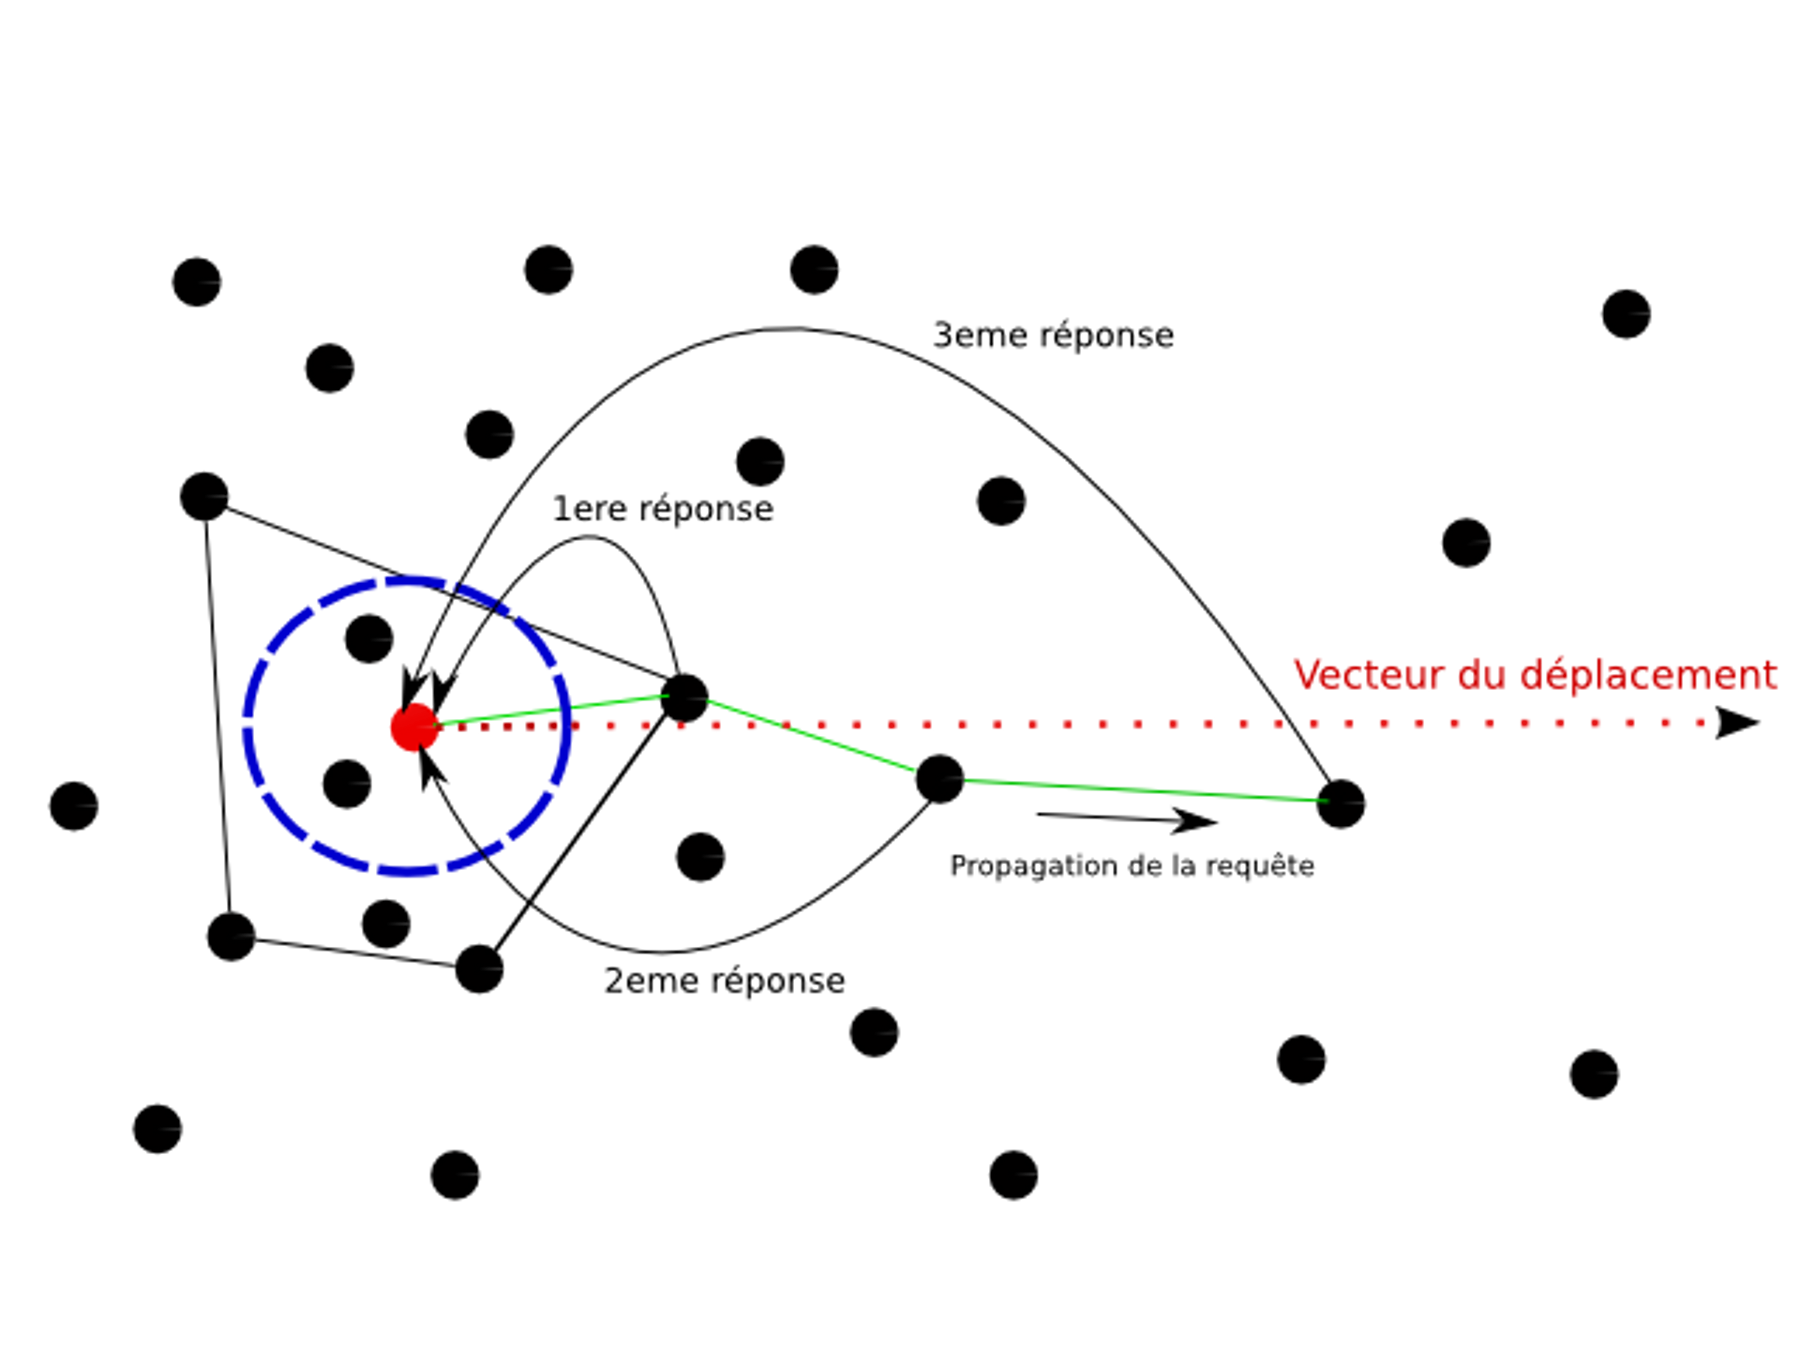
\includegraphics[scale=0.3]{./Ressources/Images/propagation_algo.png}\\
        \label{Propa_Algo}
        \end{figure}
	\end{column}
	\end{columns}

  \end{frame}

  \section{Les améliorations}
  \begin{frame}
	Durant le stage, plusieurs solutions ont été implémentées:
	\begin{itemize}
		\pause\item Le cache pour les zones denses
		\pause\item Le préchargement amélioré des données
	\end{itemize}
	\pause D'autres solutions ont été étudiées, mais sans être implémentées.
	\begin{itemize}
		\item Mouvements de groupe
		\item Connaissance des routes entre les zones denses
	\end{itemize}
  \end{frame}

  \begin{frame}
	Différentes métriques utilisées pour analyser les résultats:
	\begin{itemize}
		\item Nombre de messages
		\item Cohérence de la topologie
		\item Cache Hit et Miss (pour le cache)
	\end{itemize}
	\vspace{5mm}
	En fonction du degré de mobilité.
  \end{frame}

  \section{Le cache pour les zones denses}
  \begin{frame}
	\center{Le cache des zones denses}
	\vspace{1cm}
	\begin{itemize}
		\item Explications sur le cache des zones denses
		\item Les résultats 
		\item Conclusion sur le cache
	\end{itemize}
  \end{frame}
  
  \subsection{Explications du cache pour les zones denses}
  \begin{frame}
	Comment fonctionne le cache?
	\begin{itemize}
 		\item Chaque nœud de l'environnement a un cache.
		\item Il est utilisé seulement par les nœuds en état \textbf{E}(xploring).
		\item Deux types de cache mis en place (retour simple et retour multiple).
	\end{itemize}
  \end{frame}

  \begin{frame}
	Trois types de recherche dans le cache:
	\vspace{7mm}
	\tiny{
	\begin{table}
  		\begin{center}
    		 \begin{tabular}{|c|c|c|c|}
      		 \hline
      		 N & Critère de sélection & Avantages & Inconvénients\\
      		 \hline
        	 1 & Comparaison distances & Simplicité & Distance~$\ne$~utile, aide pas enveloppe\\
        	 2 & Aide enveloppe & + Enveloppe OK & - bon règles Solipsis\\
        	 3 & Zone de connaissance & Simplicité & aide pas enveloppe\\
      		 \hline
    		 \end{tabular}
  		\end{center}
	\end{table}
	}
  \end{frame}
 
  \begin{frame}
  	\only{\begin{figure}
        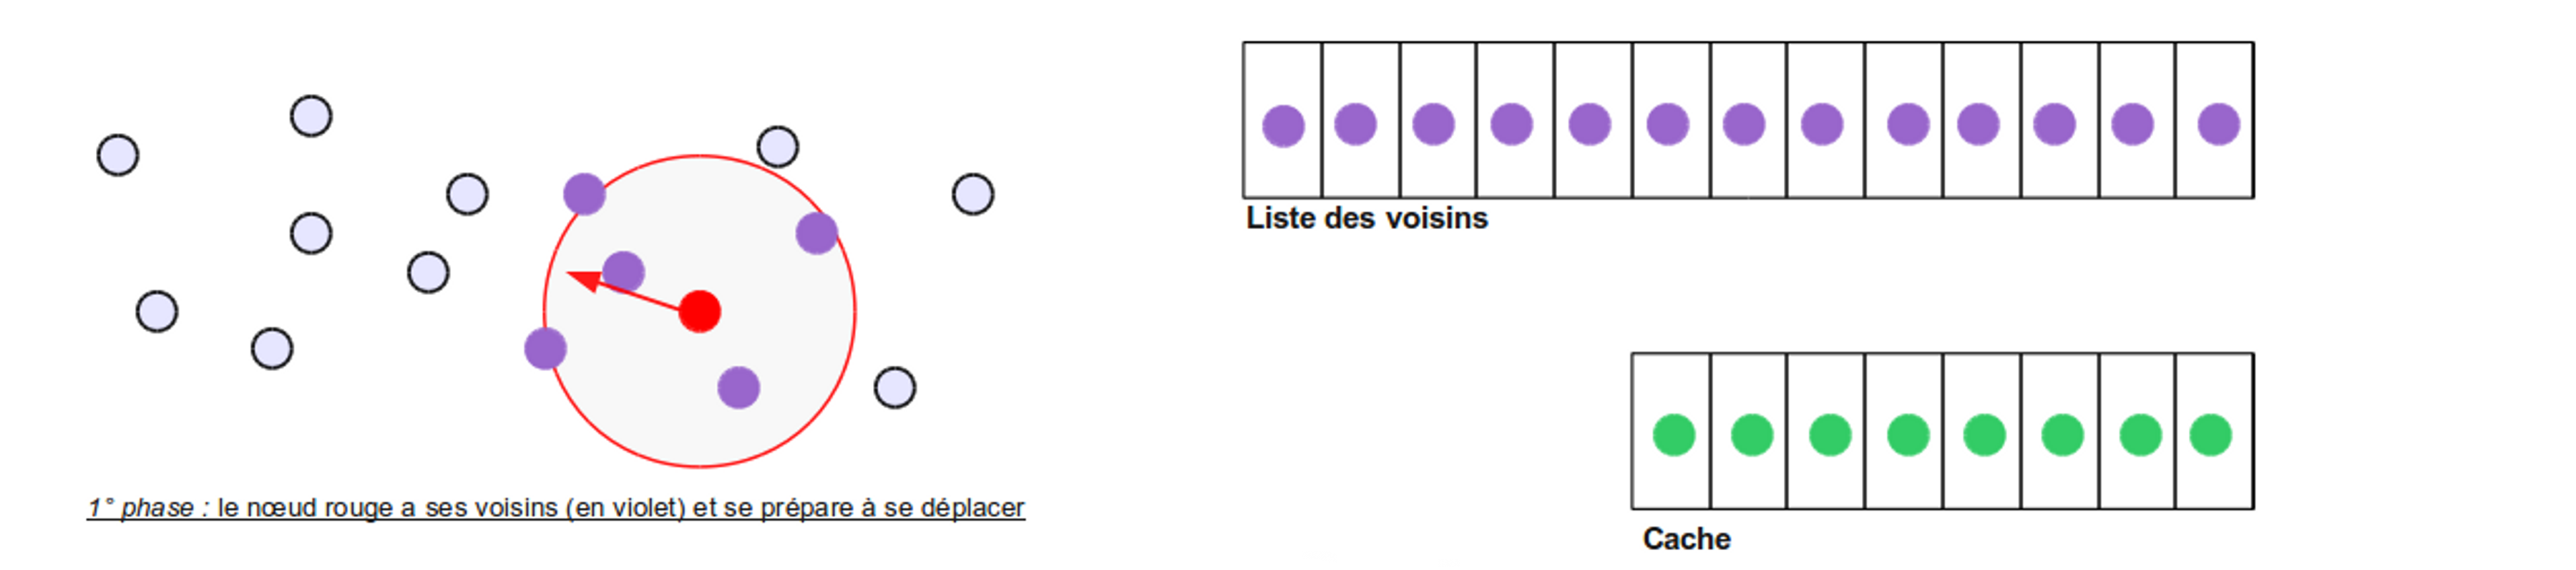
\includegraphics[scale=0.08]{./Ressources/Images/etape1.png}\\
        \label{etape1}
        \end{figure}}
  \end{frame}
	
  \begin{frame}	
  	\only{\begin{figure}
        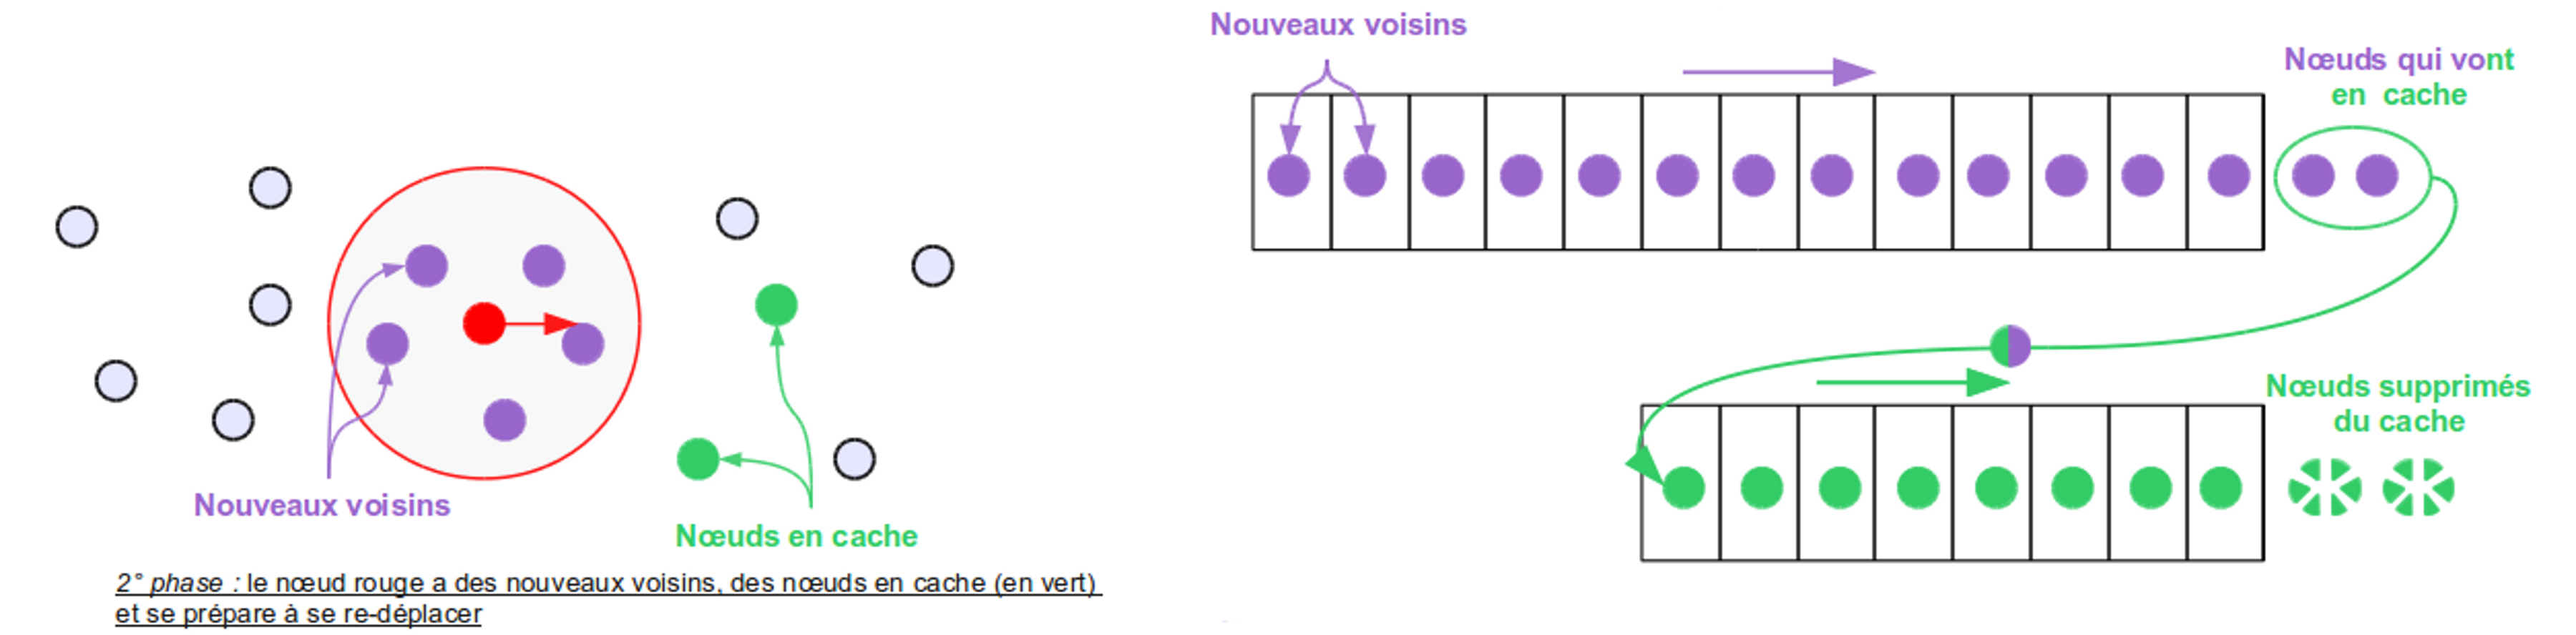
\includegraphics[scale=0.08]{./Ressources/Images/etape2.png}\\
        \label{etape2}
        \end{figure}}
  \end{frame}

  \begin{frame}
  	\only{\begin{figure}
        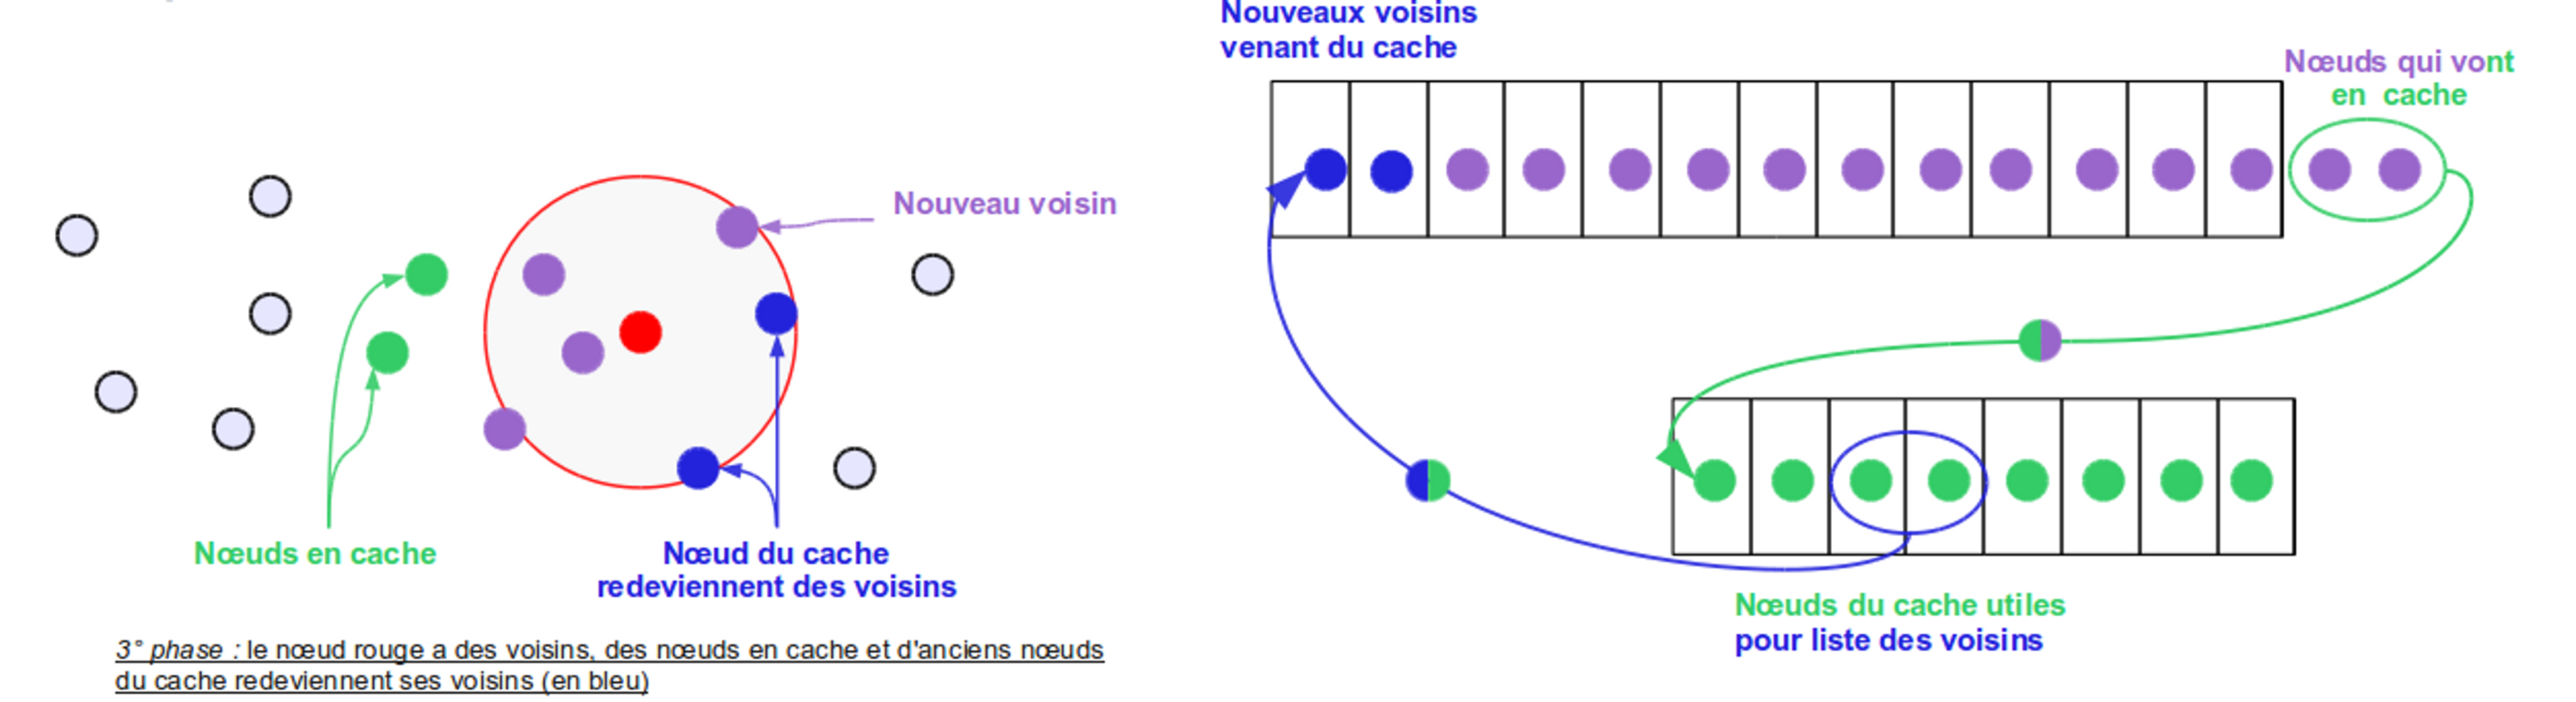
\includegraphics[scale=0.08]{./Ressources/Images/etape3.png}\\
        \label{etape3}
        \end{figure}}


  \end{frame}

  \begin{frame}
	Différents mécanismes pour le cache:
	\begin{itemize}
		\item Mise à jour des données du cache
		\item Contact un nœud du cache s'il est là depuis longtemps
		\item Aide les nœuds voisins lors de recherche de nœud	
	\end{itemize}
  \end{frame}

 
  \subsection{Résultats pour le cache}
  \begin{frame}
	\begin{columns}
         \begin{column}{5cm}
          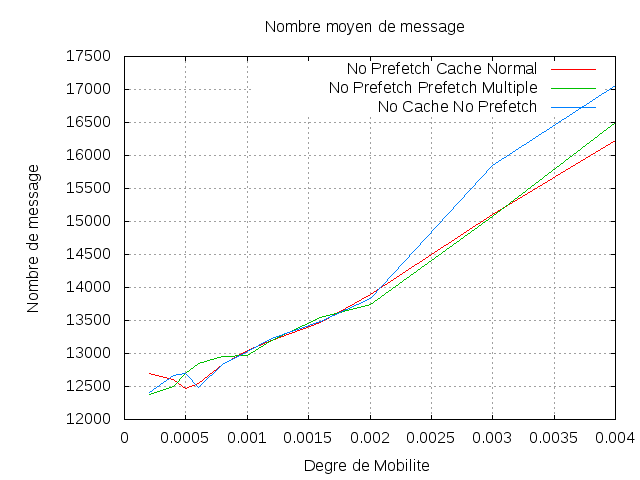
\includegraphics[scale=0.25]{./Ressources/Images/Courbes_Final_Rapport/Nombre_Messages_Caches.png}\\
         \end{column}
         \begin{column}{5cm}
          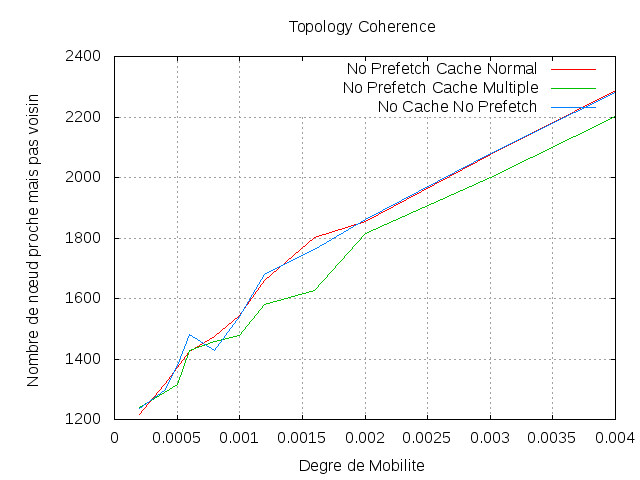
\includegraphics[scale=0.25]{./Ressources/Images/Courbes_Final_Rapport/Topology_Coherence_Caches.png}\\
         \end{column}
        \end{columns}


  \end{frame}

  \begin{frame}
  	Résultats des deux versions du cache en fonction d'une version sans le cache activé:
	\begin{table}[!h]
  		\begin{center}
    		\begin{tabular}{|c|c|c|c|}
      		\hline
      		Solution & Cohérence topologie & Nombre de messages \\
      		\hline
      		Cache simple & Équivalente &  5\% de msg en moins\\
      		Cache multiple & 3\% de gains &  5\% de msg en moins\\
      		\hline
    		\end{tabular}
  		\end{center}
  		\label{tab:config1}
	\end{table}
	
  \end{frame}
	
  \subsection{Conclusion sur le cache des zones denses}
  \begin{frame}
  	La mise en place du cache permet:\\
	\begin{itemize}
		\item d'économiser des messages.\\
		\item d'améliorer la cohérence de la topologie.\\
	\end{itemize}
	\vspace{5mm}
	Amélioration possible en testant toutes les combinaisons de paramètres (mise à jour, contact d'un nœud, taille du cache, etc).\\
  \end{frame}



  \section{Le préchargement amélioré des données}
  \begin{frame}
	\center{Le préchargement amélioré des données}
	\vspace{1cm}
	\begin{itemize}
		\item Explications sur le préchargement amélioré
		\item Les résultats 
		\item Conclusion sur le préchargement
	\end{itemize}
  \end{frame}

  \subsection{Explications du préchargement amélioré}
  \begin{frame}
	\textbf{Situation:} Le préchargement de Blue Banana prend tous les nœuds, à bonne distance, dans le cône.\\
	\vspace{5mm}
	\textbf{Problème:} Des nœuds inutiles sont préchargés.\\
	\vspace{5mm}
	\textbf{Solution:} Choisir plus finement les nœuds qui vont être sélectionnés.\\
	\vspace{5mm}
	\textbf{Comment:} Regarder la direction des nœuds et leur vitesse.\\
  \end{frame}

  \begin{frame}
	\begin{columns}
         \begin{column}{5cm}
	 Préchargement si:
          \begin{itemize}
		\item l'angle du nœud est proche du nœud courant
		\item \textit{Somme des normes des vecteurs~$\ge$~Norme du vecteur de prefetch +/- $\Delta$}
		\item l'angle du nœud n'est pas proche du nœud courant mais sa norme est inférieure à celle du nœud courant
	  \end{itemize}
	 \end{column}
         \begin{column}{6cm}
          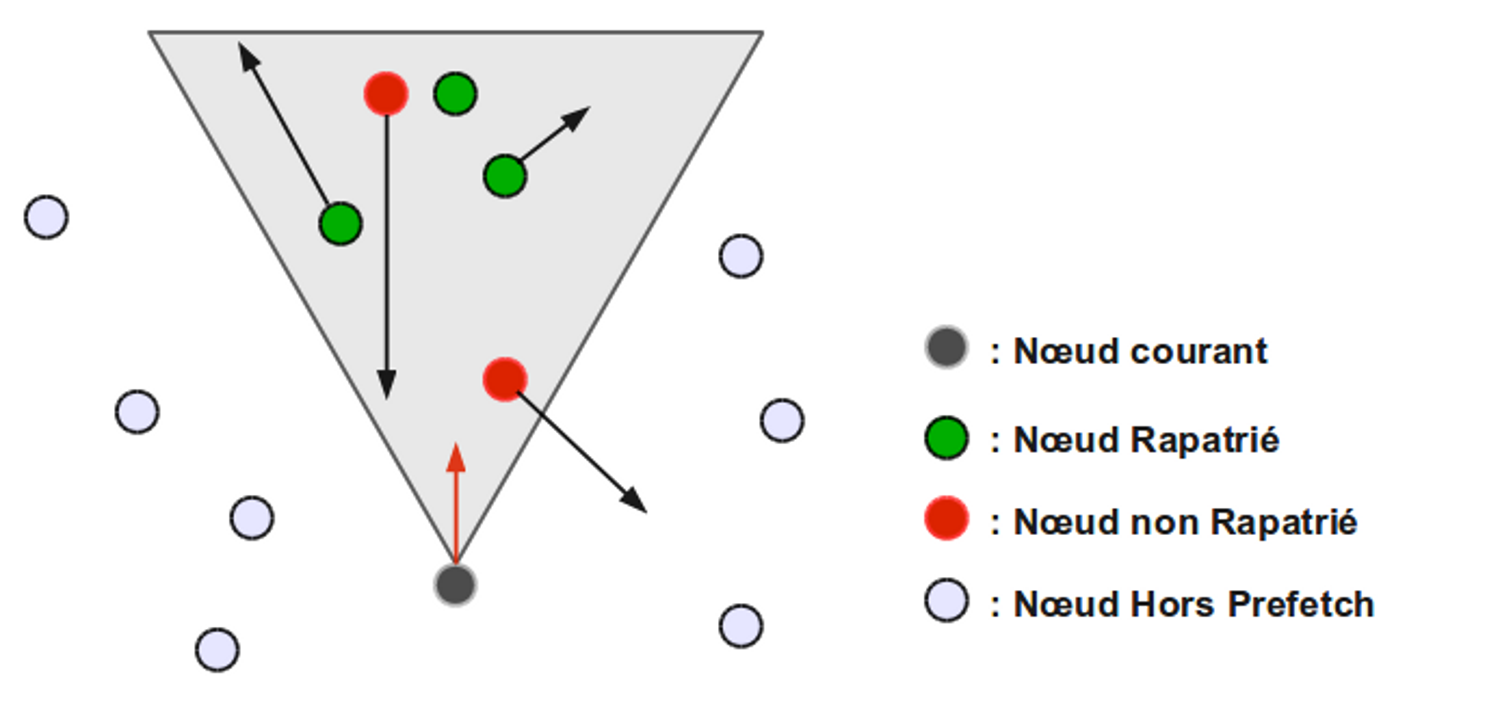
\includegraphics[scale=0.11]{./Ressources/Images/prefetchaV1.png}\\
         \end{column}
        \end{columns}

  \end{frame}
	
  \subsection{Résultats pour le préchargement amélioré}
  \begin{frame}
	\begin{columns}
         \begin{column}{5cm}
          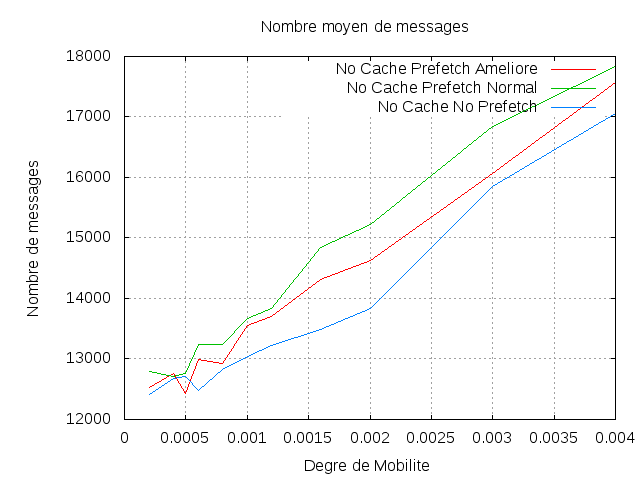
\includegraphics[scale=0.25]{./Ressources/Images/Courbes_Final_Rapport/Nombre_Messages_Prefetchs.png}\\
         \end{column}
         \begin{column}{5cm}
          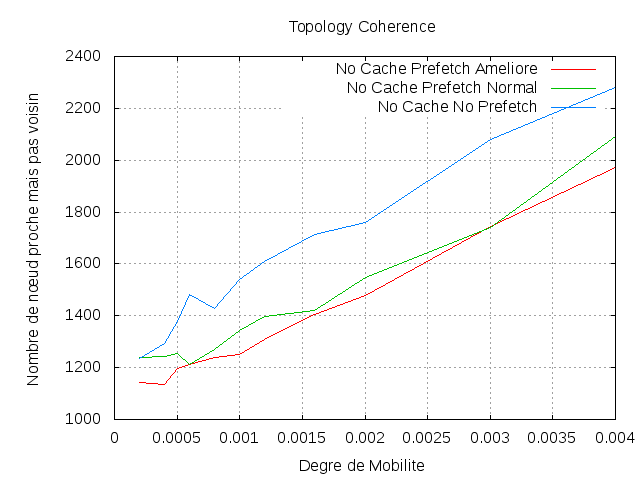
\includegraphics[scale=0.25]{./Ressources/Images/Courbes_Final_Rapport/Topology_Coherence_Prefetchs.png}\\
         \end{column}
        \end{columns}
  \end{frame}
	
  \begin{frame}
	 Résultats des différents préchargements en comparaison à une version sans le préchargement activé:
        \begin{table}[!h]
                \begin{center}
                \begin{tabular}{|c|c|c|c|}
                \hline
                Solution & Cohérence topologie & Nombre de messages \\
                \hline
                Préchargement Normal & 15\% de gains &  8\% de msg en plus\\
                Préchargement Multiple & 16\% de gains &  4\% de msg en plus\\
                \hline
                \end{tabular}
                \end{center}
                \label{tab:config1}
        \end{table}
  \end{frame}

  \subsection{Conclusion sur le préchargement amélioré}
  \begin{frame}
	Le préchargement amélioré permet:
	\begin{itemize}
		\item d'économiser des messages par rapport au préchargement normal.\\
		\item d'améliorer légèrement la cohérence de la topologie.\\
	\end{itemize}
	\vspace{5mm}
	Possibles améliorations du préchargement en regardant d'autres paramètres, comme la distance avec les nœuds.
  \end{frame}
	
  
  \section{Conclusion}
  \begin{frame}
	Les différentes solutions ont permis d'améliorer la réactivité des réseaux pair à pair pour les MMOGs.\\
	Meilleur cohérence de la topologie et moins de message que dans Blue Banana.
  \end{frame}
	

  \begin{frame}
	\begin{center}
	Merci.\\
	\vspace{1cm}	
	Questions?
	\end{center}
  \end{frame}  

  \end{document}
